\section{Test cases and Results}
The proposed solar PV detection was implemented using python language.
Two power system are tested. There two test cases are based on four bus system and CIGRE Task Force C6.04.02 paper\cite{b3}.

\subsection{Test cases}

\subsubsection{four bus system}

The one line diagram of the four bus system is shown in Fig.~\ref{fig.4_bus_system}.

\begin{figure}[h!]
  \center
  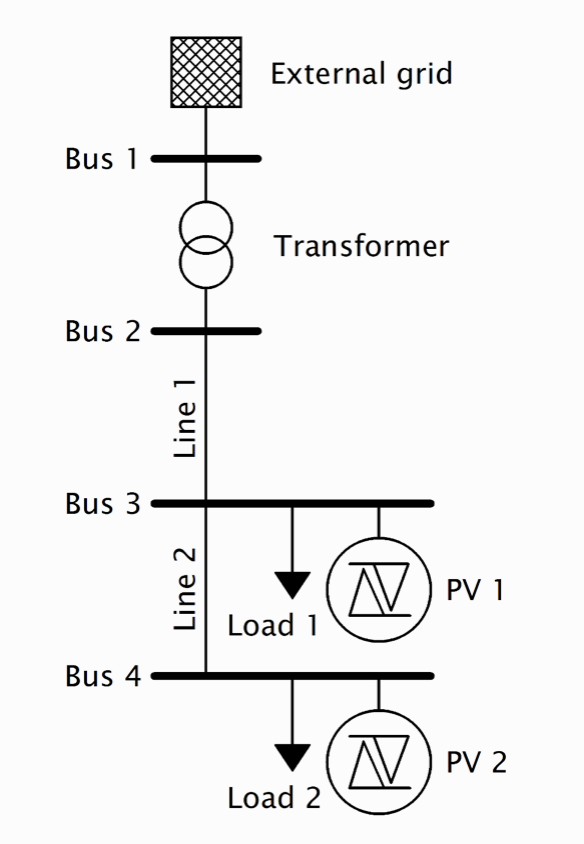
\includegraphics[scale=0.5]{images/four_bus_system.png}
  \caption{four bus system}
  \label{fig.4_bus_system}
\end{figure}

Table \ref{tab.res_1} shows the results. From the table, \ref{tab.res_1} it can be seen that the proposed method can predict perfectly location of solar PV.

\begin{table}[h]
  \caption{Results of 4 bus system}
  \begin{tabular}{cc}
    \hline
  {[}random PV location at bus (size of PV kW){]} & Solar PV detection \\
  \hline
  {[}1(10){]}                                     & {[}1(8){]}         \\
  {[}1(10), 2(20){]}                              & {[}1(9), 2(17){]}\\
  \hline
  \end{tabular}
\label{tab.res_1}
\end{table}

\subsubsection{CIGRE system}



\begin{figure}[h!]
  \center
  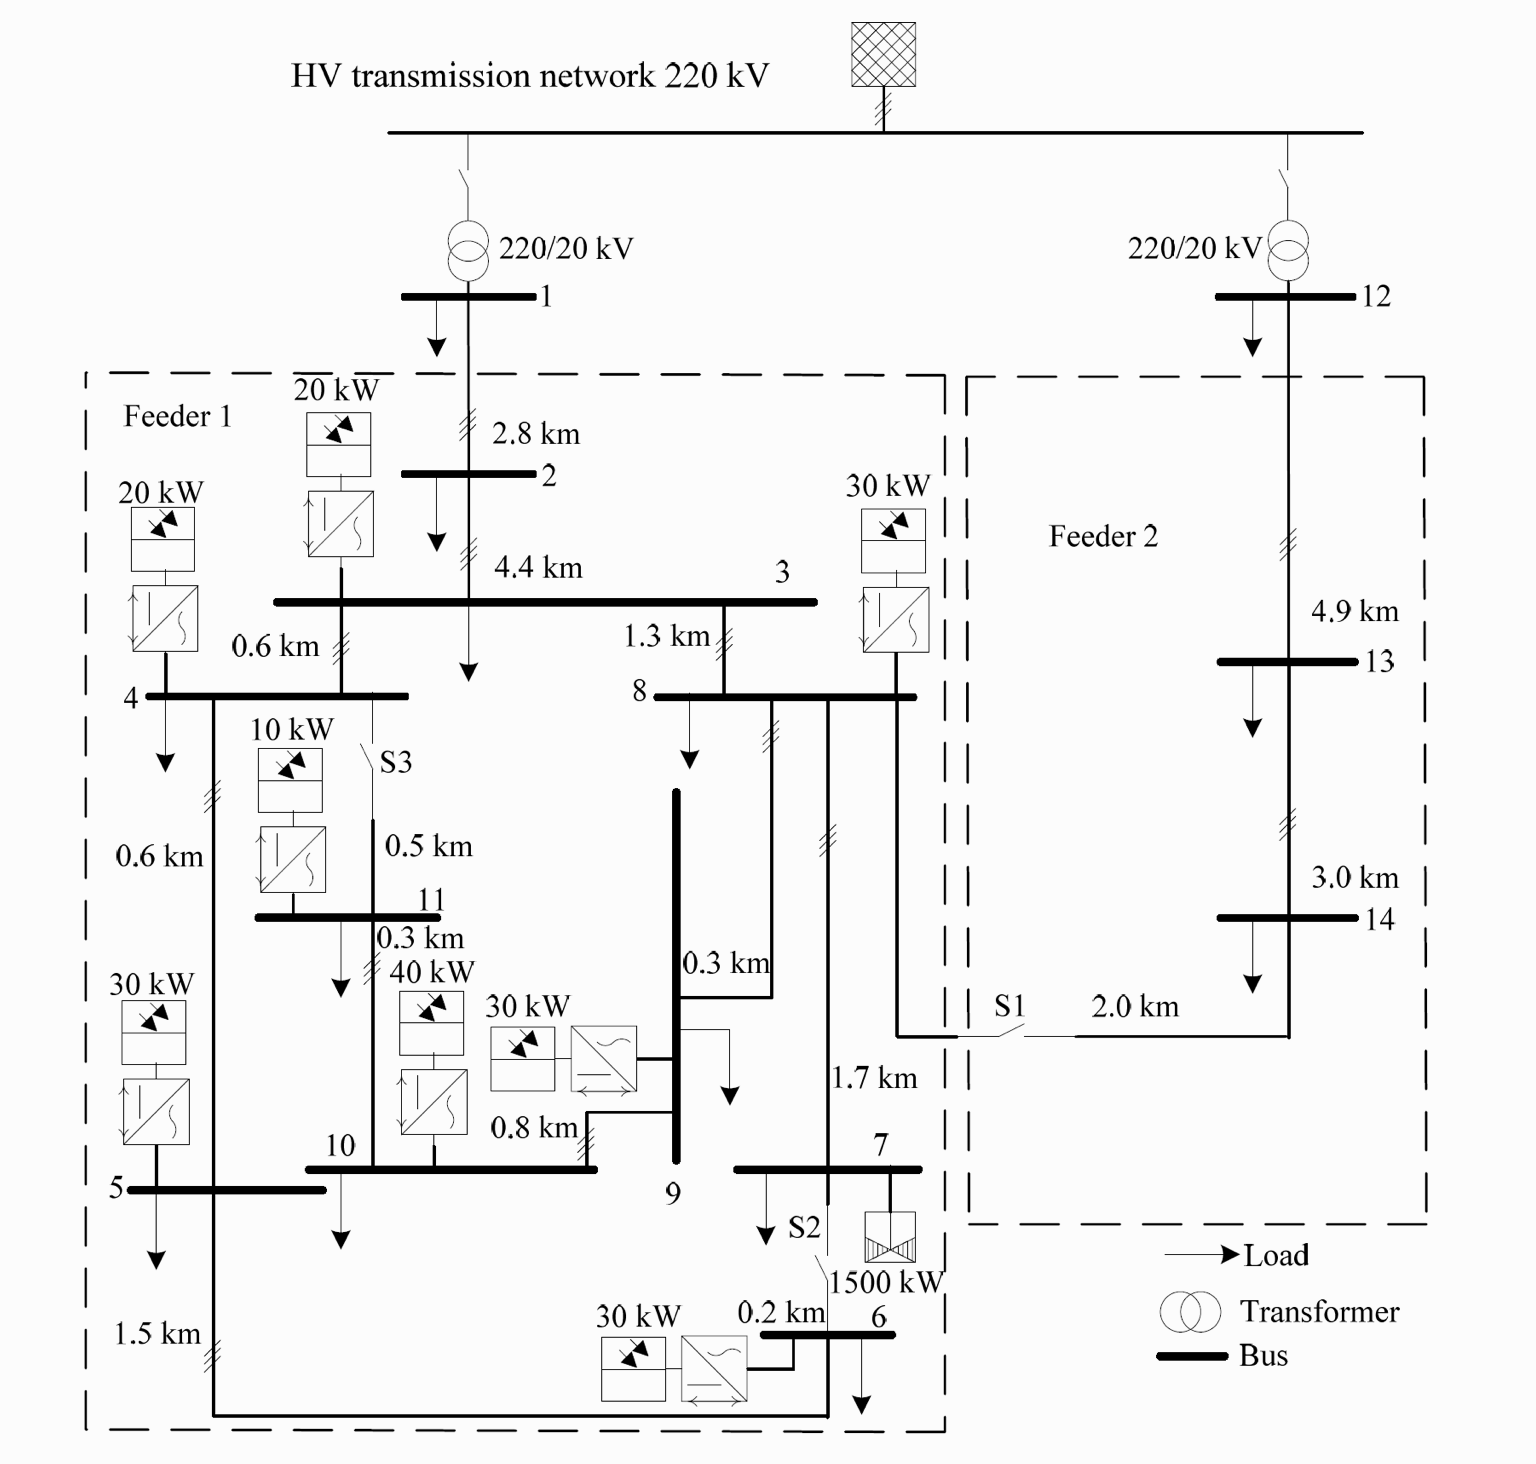
\includegraphics[scale=0.25]{images/CIGRE_network.png}
  \caption{CIGRE network}
  \label{fig.CIGRE_network}
\end{figure}


Table \ref{tab.res_2} shows the results. From the table, \ref{tab.res_2} it can be seen that the proposed method can predict perfectly location of solar PV.

\begin{table}[h]
  \caption{Results of CIGRE}
  \begin{tabular}{cc}
    \hline
  {[}random PV location at bus (size of PV kW){]} & Solar PV detection \\
\hline
  {[}1(10){]}                                     & {[}1(8){]}         \\
  {[}1(10), 2(20){]}                              & {[}1(9), 2(17){]}\\
  \hline
  \end{tabular}
  \label{tab.res_2}
\end{table}



\subsection{Results}
